\chapter{Background}\label{chap:background} \minitoc

\section{Stream processing as a superset of batch processing} \label{sec:stream-superset}

Batch processing is the processing of data grouped by batches. A batch is a collection of data points that have been grouped by certain criteria. Examples of such criteria could be \textit{"all the transactions from the past two months"}, \textit{"the last million transactions"} or even \textit{"all the transactions made by an user until now"}. Batch data sets are known as static data \cite{Martin-Batch-Defin}. An example application of such a technique would be processing all the keywords searched for in the google search engine by grouping the results by keyword and counting how many times a keyword was searched for trend analysis purposes. Batch processing is the oldest paradigm between batch and stream processing. Historically speaking, Apache Hadoop \cite{borthakur2007hadoop} \cite{Hadoop} \cite{ApacheHadoop} was one of the first widely known frameworks for large-scale batch processing, created in 2005. Hadoop uses a distributed computation framework or programming model called MapReduce \cite{MapReduce}. This paradigm applies a map function that processes key/value pairs and generates sets of intermediate ones, ultimately merging all intermediate values
using a reducer function. To do this they read and write from disk on intermediate steps, which makes it inefficient for applications that reuse working sets of data across multiple parallel operations (\textit{e.g.} iterative Machine Learning algorithms). Nearly a decade later, Apache Spark \cite{ApacheSpark} \cite{Spark} was released.
Spark retains the scalability and fault tolerance of MapReduce but introduces Resilient Distributed Datasets (RDDs) \cite{SparkRDDs}. An RDD is a read-only collection of objects partitioned across a set of machines that can be rebuilt if a partition is lost.
Additionally, Spark processes data in random access memory (RAM), while Hadoop MapReduce persists data to the disk after a map or reduce action. Thus, Spark achieves lower processing times. 

On the other hand, stream processing refers to the processing of data streams. A data stream is essentially a continuous or unbounded data set. This data needs to be processed sequentially and incrementally on a event-by-event basis or over sliding windows. Streaming data includes a wide variety of data such as logs generated by customers using mobile or web applications, sensor data from Internet-of-Things (IoT) devices or credit card transactions. This is in contrast to batch processing which works on a finite data set. This distinction is important since some aggregations are very hard and even impossible to compute with 100\% accuracy for several use cases in an efficient manner on unbounded data sets. An example of such is counting distinct elements that flow through the data stream. An immediate solution would be to create a regular set of items or strings and have its length be the number of distinct elements processed. However, this approach is not very efficient and has a linear memory usage growth regarding the number of distinct elements. Therefore, as the number of distinct elements approaches large orders of magnitude we run out of memory.

In order to provide a streaming solution, Apache Spark created the Spark Streaming \cite{SparkStreaming} module. Being a batch system in its core, Spark implements streaming as micro-batching \cite{SparkStreamingPaper}. This approach handles streaming data by grouping incoming events into very small batches. Then, in order to process the entire defined window of data, it joins all micro-batches into a larger one and performs the desired computations. However, this creates an artificial barrier that does not truly exist in the streaming context. More than conceptually different from a true stream processing system, processing a stream in a batch fashion, even if in small ones, presents some issues. First, since we are indeed working with batches, results will never be updated in real-time per event being processed. For example, if we use a batch size of 100 events, the system would only produce accurate results every 100 events. To handle system inactivity usually these micro-batch systems also have the notion of updating the aggregations with incomplete batches, if no event has entered the system after a pre-specified time period has elapsed. As such, micro-batching was created as a natural implementation of stream processing using the available batch processing systems of the time, but can not be considered true stream processing.

The Venn diagram \ref{fig:stream-superset} from a blog post by Ververica \footnote{https://www.ververica.com/blog/batch-is-a-special-case-of-streaming} illustrates the relation of both processing techniques. A data stream is unbounded or infinite while a bounded data stream has a beginning and an end. Using these definitions, the concept of an unbounded data stream contains that of a bounded data set. That is, from an infinite stream, it is possible to fix a left and right limits in order to obtain a bounded and finite data set. This relation is visible in Figure \ref{fig:unbounded-bounded-superset} from the same blog post.

\begin{figure}[!htb]
    \begin{center}
      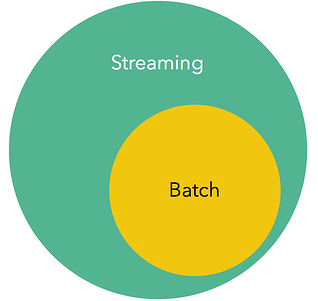
\includegraphics[scale=0.5]{figures/streaming-subset-batch.png}
      \caption{Stream processing as a superset of batch processing}
      \label{fig:stream-superset}
    \end{center}
\end{figure}

\begin{figure}[!htb]
    \begin{center}
      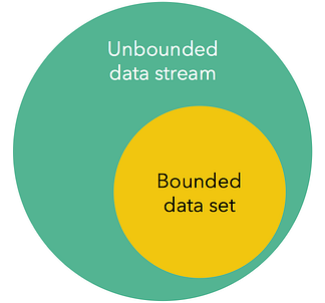
\includegraphics[scale=0.5]{figures/unbounded-superset-bounded.png}
      \caption{Unbounded data streams as a superset of bounded data sets}
      \label{fig:unbounded-bounded-superset}
    \end{center}
\end{figure}


In Section 2.2 we will cover exactly how an unbounded data set (also known as a data stream) can be converted into a bounded data set with the use of windows.

\section{From unbounded streams to finite data sets} \label{sec:windows}

In Section 2.1 we have defined a data stream as an unbounded data set. But what exactly are the issues of working with an infinite stream of data? Why might we need to convert it into a bounded data set and how to do so? In this Section, we will analyze such issues and present streaming windows as the solution.

% boundless aggregations no need for windows
Computations over an unbounded data set are possible. For example, computing the \textit{average} of an event's field for all incoming events is computationally trivial: we need only to store the total number of events (one integer) and the current total sum (one double) of all events arriving to the system. However, is this boundless average over the stream of events useful? While in some scenarios it may be, more often than not we would like to introduce some boundaries into our computations. For instance, consider the monitoring of machines spread out across multiple racks in a large data center and its temperatures. Assume that temperatures measured across all racks are sent to a monitoring system in the form of a data stream. The average temperature of a machine over an infinite period (\textit{i.e.} since the machine was deployed) is of little value for detecting if the equipment is currently overheating, and to trigger the appropriate action to prevent a failure. In this scenario, an average of the temperatures per rack and for the last 5 minutes allows for more actionable context, in this case identifying a likely-to-fail rack. To obtain such insight requires computing the average over the last 5 minutes' worth of data, effectively defining a begin and end --- \textit{i.e.} all the data between the current timestamp in minutes \textit{t} and \textit{t-5}. By creating such a conceptual range, we realize that in practice we need a bounded data set. Partitioning an infinite data stream to obtain such a finite data set is made through the use of windows.

\subsection{Sliding Windows}

Botan et. al \cite{Botan-SECRET} formally define a window as:

\begin{definition}
A window W over a stream S is a finite subset of S"
\end{definition}

% 2 dimensions of windows
Windows can be categorized by two dimensions: the window size $W$ and the sliding step size $S$. Windows can be defined as tuple or time-based. Tuple-based windows are windows whose size is defined by \emph{number} of items contained in the window, whereas time-based windows are windows whose size is defined by the total \emph{time} a window can store. For instance, a tuple-based window of size $10^3$ tuples will store exactly $10^3$ items. In contrast, a time-based window storing the last 5 minutes of events can contain a varying number of tuples but will always keep the events arrived in the last 5 minutes. A window slides over incoming data and groups it, enabling us to compute aggregations over a defined and bounded set of events. The step size \textit{S} of a windowing technique is formally defined as the distance between consecutive windows \cite{Botan-SECRET}. This means that two consecutive windows W\textsubscript{1} and W\textsubscript{2} are exactly \textit{S} units away. As mentioned, these units can be units of time or a number of tuples.

Windows can also be characterized by how they move across data, \textit{i.e.}, how the step $S$ is defined. The three most common ways are: true sliding, stepping or tumbling windows. A true sliding window is a window with an unitary step, i.e., where $S = 1$. At each step, the window advances one unit, which may be one event for tuple-based steps, or one time-unit whether that is in milliseconds, seconds, days, weeks or another magnitude of time, measured based on the system clock or event time. Such a true sliding movement can be observed in Figure \ref{fig:sliding-window} with a tuple-based window of size \textit{W} of three tuples and unitary step. 

\begin{figure}[!htb]
    \begin{center}
      \hspace*{0.6in}
      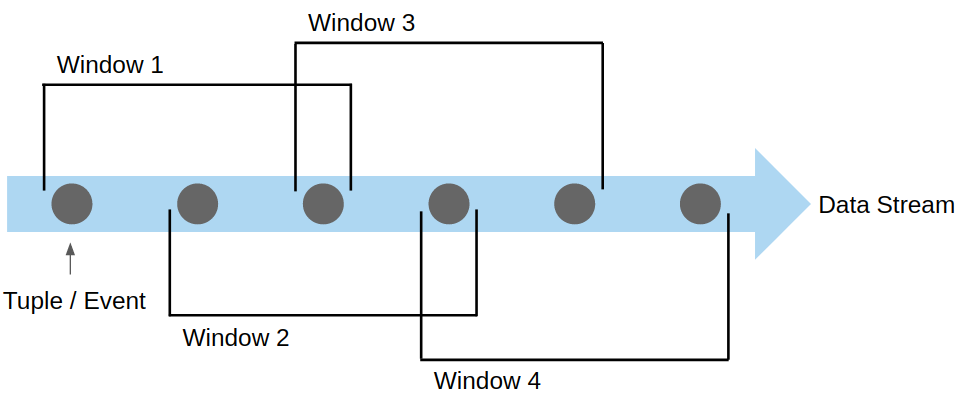
\includegraphics[scale=0.35]{figures/sliding.png}
      \caption[True sliding window]{True sliding window, W=3, S=1}
      \label{fig:sliding-window} 
    \end{center}
\end{figure} 

% stepping windows (per x units over Y window size)
% stepping: step > 1 < window size
A stepping window behaves exactly like a true sliding one but the step size \textit{S} is not unitary, \textit{i.e.}, $S > 1$. In other words, a stepping window is defined by any window size \textit{W} and steps \textit{S} greater than a unit. Figure \ref{fig:stepping-window} represents a stepping tuple-based window of size \textit{W} of three and a stepping size \textit{S} of two.

\textcolor{red}{TODO change all window drawings to a not horrendous style}

\begin{figure}[!htb]
    \begin{center}
      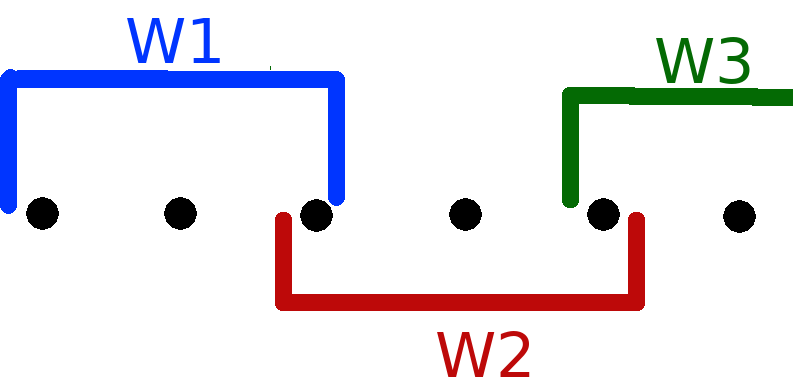
\includegraphics[scale=0.3]{figures/stepping.png}
      \caption[Stepping window]{Stepping window, W=3, S=2}
      \label{fig:stepping-window}
    \end{center}
\end{figure}

% tumbling: step = window size
A tumbling window is a window with a stepping size as large as the window, \textit{i.e.}, $S = W$. Hence, tumbling windows partition the stream into non-overlapping chunks with the same size. Since the intersection of different tumbling windows is always empty, each event is said to belong to exactly one tumbling window. An example of a tumbling window can be seen in Figure \ref{fig:tumbling-window} with a tuple-based window of size \textit{W} of three and an equally large step size \textit{S}.

\begin{figure}[!htb]
    \begin{center}
      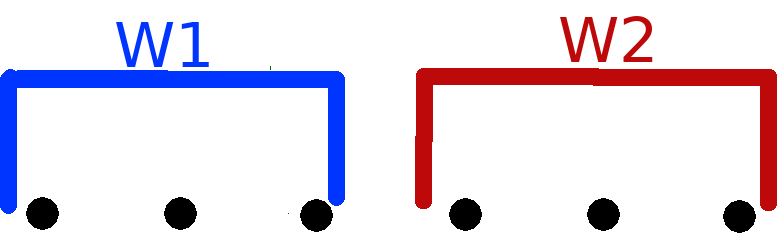
\includegraphics[scale=0.3]{figures/tumbling.png}
      \caption[Tumbling window]{Tumbling window, W=S=3}
      \label{fig:tumbling-window}
    \end{center}
\end{figure}

The mathematical expression below summarizes our categorization of sliding windows.
\begin{equation} 
\label{math:windows}
  Sliding\ window \,\, of \,\, size \,\, W, \,\, step \,\, S =
    \begin{cases}
      true \,\, sliding & \text{if \textit{S}=1}\\
      stepping & \text{if \textit{S}>1}\\
      tumbling & \text{if \textit{S}=\textit{W}}
    \end{cases}
\end{equation}

For the scope of this Thesis, we will work under a tuple-based true sliding window framework. However, as explained in Section \ref{sec:ft-monitoring}, despite focusing on tuple-based true sliding windows, our approach is just as valid for time-based windows and other step values as well.

\section{Aggregations over data} \label{sec:aggregations}

An aggregation --- also known as a fold, reduce or accumulate function --- is an operation that reduces a collection of values into a single one. Examples of such are the computation of data set sums, minima, averages or the number of distinct elements (cardinality). An aggregation may be exact or approximate. Exact aggregations compute a value from a sequence of elements, where no error or loss of resolution exists. On the other hand, approximate aggregations have an error margin to the associated aggregation value which is usually controllable by adjusting a set of parameters. 
Approximate aggregations are most useful in situations where memory is limited, the volume of data to process is large and/or computing the exact aggregation can not be done in useful time. Thus, approximate aggregators trade precision of results for efficient time and space usage. In Section \ref{sec:pds} we explore approximate aggregators that make such a trade-off.

Aggregations are present in most programming languages and frameworks. Quoting from the Java programming language documentation on the \textit{Stream.reduce()} method \cite{Java13StreamReduce}: 
\textit{"A reduction operation (also called a fold) takes a sequence of input elements and combines them into a single summary result by repeated application of a combining operation"}. Similarly, the MapReduce \cite{MapReduce} paradigm consists of first applying \textit{map} steps to the collection of data and then a \textit{reduce} one. \textit{Map} tasks will transform each item as desired and the \textit{reduce} task will merge the collection into a single value. Reduce methods make use of a \textit{combine} function and recursively apply it. The \textit{combine} function takes the current aggregation value and combines it with the next item in the set, returning the new aggregated state. Doing this recursively for each item in the collection results in a single value: the aggregate value. The combine function is here on forward represented by $\oplus$ and the identity or neutral element of the aggregation by $\overline{\theta}$.

\subsection{Sliding Window Aggregations}

While some aggregations can be computed on an infinite data set, often we want to compute these over a finite one. As we have seen in Section \ref{sec:windows}, we can obtain a bounded data set from a data stream by applying windowing techniques. When doing so, we obtain a finite data set denoted as a sliding window and compute aggregations over it. Tangwongsan \emph{et. al} define such aggregations over sliding windows as Sliding Window Aggregations (SWAGs) \cite{Tangwongsan-Sliding-Window-Aggregation-Algorithms}. As an example of a SWAG, consider the data center temperature monitoring problem from Section \ref{sec:windows}. In this example, we wanted to compute the average temperature per rack in the data cencer in the last 5 minutes. If we translate this SWAG into streaming SQL following a similar syntax to the one provided by Apache Flink \cite{ApacheFlink} we would get:

\begin{verbatim}
SELECT rack_id, AVG(temperature)
FROM Temperatures
GROUP BY TUMBLE(timestamp, Time.minutes(5), rack_id)
\end{verbatim}

In the query above, the
\texttt{TUMBLE(timestamp, Time.minutes(5), rack\_id)} statement groups incoming data using time-based tumbling windows of 5 minutes duration, using the \texttt{timestamp} field to evict events not in this time interval. The resulting list of rows has \texttt{rack\_id} as its key and as corresponding value a list of temperatures, from the past 5 minutes. Finally, for each rack and its list of temperatures, we compute an \texttt{AVG} aggregation, resulting in the average temperature per rack in the past 5 minutes. Note that this is very similar to any aggregation made in a standard Database Management System (DBMS). The main difference is that in standard SQL the \texttt{GROUP BY} clause includes only the columns on which the data will be grouped while in streaming SQL the \texttt{GROUP BY} also specifies the type of window used (\textit{e.g.} in this case, a tumbling window).


\subsection{Sliding Window Aggregation Algorithms} \label{sec:back-swag-algs}

A sliding window aggregation algorithm allows the computation of an exact or approximate aggregation over a sliding window. A SWAG algorithm may restrict the set of computable aggregations based on their properties. Different SWAG algorithms use different data structures for the window contents and the incremental aggregation state.

Two of the most basic SWAG algorithms are \textit{Recalculate-From-Scratch (RFS)} and \textit{Subtract-On-Evict (SOE)}. Recalculate-From-Scratch (RFS) is the simplest and most general SWAG algorithm. As the name suggests, this algorithm recomputes the aggregation over the entire window for each update. For instance, the computation of a sum over a sliding window using RFS means that whenever the window changes all elements are summed. This approach works for every aggregation. However, given \textit{n} as the window size, this algorithm takes \textit{O(n)} space and time complexity which makes it unfit in most scenarios of large scale data processing. Recall that the combine function is represented by $\oplus$ and the identity or neutral element of the aggregation by $\overline{\theta}$. Pseudocode for the Recalculate-From-Scratch algorithm is shown in Algorithm \ref{pseudo:rfs}.
  

\begin{algorithm}
    \caption{Recalculate-From-Scratch insert, evict and query methods}
    \label{pseudo:rfs}
    \begin{algorithmic}[1]
        \Function{query}{vals}
            \State $agg\gets\overline{\theta}$
            \ForEach {$v \in vals$}
                \State $agg \gets agg \oplus v$
            \EndFor
            \State \Return $agg$
        \EndFunction
        
        
        \Function{insert}{vals, v}
        
            \State $vals.pushBack(v)$
        \EndFunction
        
        
        \Function{evict}{vals}
        
            \State $vals.popFront()$
        \EndFunction
    \end{algorithmic}
\end{algorithm}

Subtract-On-Evict (SOE) on the other hand, is a SWAG algorithm that incrementally computes the aggregation value. For each element inserted or evicted from the window, the aggregation value is updated without recomputing the entire aggregation like in RFS. SOE relies on expiring the evicted elements from the aggregation state. Hence, SOE only works for \textit{invertible} aggregations, that is, a function $\ominus$ exists such that $(x \oplus y) \ominus y = x$, for all $x$ and $y$. To illustrate the differences between SOE and RFS, consider the computation of a sum aggregation over a sliding window. The total sum of the window will be the aggregation state or value. When inserting an element, the updated total window sum equals the current total sum plus ($\oplus$) the new element. The sum aggregation is considered \textit{invertible} because, when evicting an element, the new aggregation state is the total sum computed thus far minus ($\ominus$) the evicted element. With window size of \textit{n}, SOE has \textit{O(n)} space complexity and \textit{O(1)} time complexity. However, aggregations are not always invertible thus making this algorithm very restrictive and not always applicable. Algorithm \ref{pseudo:soe} shows pseudocode for SOE.

\begin{algorithm}
    \caption{Subtract-On-Evict insert, evict and query methods}
    \label{pseudo:soe}
    \begin{algorithmic}[1]
        \Function{query}{}
        
            \State \Return $agg$
        \EndFunction
        
        
        \Function{insert}{vals, v}
        
            \State $vals.pushBack(v)$
            \State $agg \gets agg \oplus v$
        \EndFunction
        
        
        \Function{evict}{vals}
        
            \State $v \gets vals.popFront()$
            \State $agg \gets agg \ominus val$
        \EndFunction
    \end{algorithmic}
\end{algorithm}

\subsection{Aggregation properties}
\label{sec:agg-properties}

On the previous Section, we presented Subtract-On-Evict as an improvement over Recalculate-From-Scratch based on the idea of aggregation invertibility. The question then becomes if there are other aggregation properties besides invertibility that must be taken into account when analyzing general stream processing algorithms.

As it turns out, besides \textit{invertibility}, other properties allow us to group aggregations in different families. Tangwongsan et al. construct Table \ref{tbl:aggregations-properties} to summarize the aggregation families and satisfying properties \cite{Tangwongsan-Sliding-Window-Aggregation-Algorithms}.

To understand these properties, we must be familiar with the \textit{combine} and \textit{query} functions. The already mentioned \textit{combine} function merges the incoming event with the incrementally computed aggregation state. The \textit{query} function is responsible for returning a result for a given query according to the current aggregation state. For instance, consider once again the use case of computing a sum aggregation over a window of data. The \textit{combine} function would be the arithmetic operator \textit{+} and would merge the current aggregation state --- \textit{i.e.} the current sum value --- with the new incoming event. The \textit{query} function would return the current aggregation state --- \textit{i.e.} return the total sum computed.


Based on the \textit{combine} and \textit{query} functions, the following are formal definitions of these properties. An aggregation is said to have:

\begin{enumerate}
    \item  an \textbf{\textit{invertible combine}} if a function $\ominus$ exists such that $(x \oplus y) \ominus y = x$, for all $x$ and $y$
    
    \item  an \textbf{\textit{associative combine}} if $(x \oplus y) \oplus z = x \oplus (y \oplus z)$, for all $x$ and $y$
    
    \item  a \textbf{\textit{commutative combine}} if $x \oplus y = y \oplus x$, for all $x$ and $y$
    
    \item  a \textbf{\textit{size-preserving combine}} if the aggregation state resulting from $\oplus$ always occupies the same space in memory
   
    \item  a \textbf{\textit{unary query}} if the query does not need any parameters --- \textit{e.g.} a membership test with a Bloom filter would require the element to test membership for as a parameter so it is not unary; returning the total sum is unary since it does not require any parameters
\end{enumerate}

\begin{table}[!htb]
\begin{center}
     \begin{tabular}{p{2cm}|p{1.5cm}p{1.5cm}p{1.5cm}p{1.5cm}p{1.6cm}|}
                 & \rotatebox{35}{\textbf{invertible combine}} & \rotatebox{35}{\textbf{associative combine}} & \rotatebox{35}{\textbf{commutative combine}} & \rotatebox{35}{\textbf{size-preserving combine}} & \rotatebox{35}{\textbf{unary query}}
                 \\
                 \hline
    \textbf{sum-like}     & \checkmark & \checkmark               & \checkmark               & \checkmark                   & \checkmark       \\
    \textbf{collect-like} & \checkmark              & \checkmark               & $\times$               & $\times$                   & ?           \\
    \textbf{median-like}  & \checkmark              & \checkmark               & \checkmark               & $\times$                   & ?           \\
    \textbf{max-like}     & $\times$              & \checkmark               & ?                   & \checkmark                   & \checkmark       \\
    \textbf{sketch-like}  & $\times$              & \checkmark               & \checkmark               & \checkmark                   & $\times$      
    \end{tabular}
    
    \end{center}
    \caption[Aggregation properties]{Aggregation properties. Checkmarks (\checkmark), crosses ($\times$), and question marks (?) indicate a property is true for all, false for all, or false for some of a given group of like operations, respectively}
  \label{tbl:aggregations-properties}
\end{table}

According to these properties, Tangwongsan et al. define five aggregation families \cite{Tangwongsan-Sliding-Window-Aggregation-Algorithms}. These are the sum, collect, median, max and sketch-like families. The sum-like family of aggregations comprises aggregations that have an invertible, associative, commutative and size-preserving \textit{combine} as well as a unary \textit{query} function. Examples of such aggregations are the sum, count, mean/average and standard deviation operations. The collect-like family of aggregations has an invertible and associative \textit{combine} function but their \textit{query} function is not always unary. For example, keeping a string concatenation aggregation is invertible and associative but not commutative nor size-preserving. While in the string concatenation case you do not need to pass any arguments to the \textit{query} function, in the case of another collect-like aggregation, for instance, keeping track of the \textit{i-th} youngest element, you need to specify in your query the parameter \textit{i} (\textit{e.g.} the 5th youngest element). Hence, their \textit{query} function is not always unary. The median-like family of aggregations contains for example the percentile operation. For example, the percentile aggregation is invertible, associative and commutative but not size-preserving and requires an argument to the \textit{query} function: the percentile to compute (\textit{e.g.} percentile 95 or 99). The max-like family comprises aggregations like the maximum or minimum, operations that are not invertible but associative and size-preserving, as well as unary from a \textit{query} function perspective. The final family, the sketch-like family, comprises aggregations that are usually solved by approximate aggregators, also called probabilistic data structures or \textit{sketches}. These aggregations can be membership queries, item frequency estimation or cardinality estimation.

The aggregation properties analyzed in this Section will be used to evaluate SWAG algorithms. Different algorithms might only apply to certain families of aggregations. This way, the multiple SWAG algorithms presented throughout this Thesis will be analyzed not only on their time and space complexity but also on the restrictions they impose regarding the aggregation' properties required. For example, under this framework, to implement Subtract-On-Evict (SOE), both the \textit{combine} $\oplus$ and its inverse $\ominus$ functions must be implemented so that SOE applies $\ominus$ to expire the evicted element from the aggregation state. Since SOE only restriction is for the aggregation to be invertible it works for the \textit{sum-like}, \textit{collect-like} and \textit{median-like} families in Table \ref{tbl:aggregations-properties}.

\section{Exponential Moving Averages} \label{sec:emas}

We talked about sliding window aggregations and algorithms to compute them. We observed that the contents of the sliding window must be stored in memory in order to evict the oldest event and discount its effect from the aggregation when a new one is inserted. In this Section we analyze Exponential Moving Averages (EMAs). EMAs process each event only upon insertion. Since there is no eviction operation to perform, we do not need to store the whole window of data.

Exponential Moving Averages (also known as Exponential Weighted Moving Averages) \cite{EMA-Everett2011} \cite{EMA-Hunter} \cite{EMA-MarcusB} are a type of reduce functions applied to a sequence of elements, one at a time in a orderly fashion, to compute a weighted average, using different weights for each element. These weights decrease exponentially with the age of the observations. In other words, EMAs give higher weights to more recent data points. Figures \ref{fig:window-weights} and \ref{fig:ema-weights} show the weights applied to past events. In a typical sliding window, events either have weight of one (inside the window) or zero (outside the window) whereas EMAs give exponentially smaller weights to older events.

\begin{figure}[!htb]
\centering
\begin{minipage}{.5\textwidth}
  \centering
      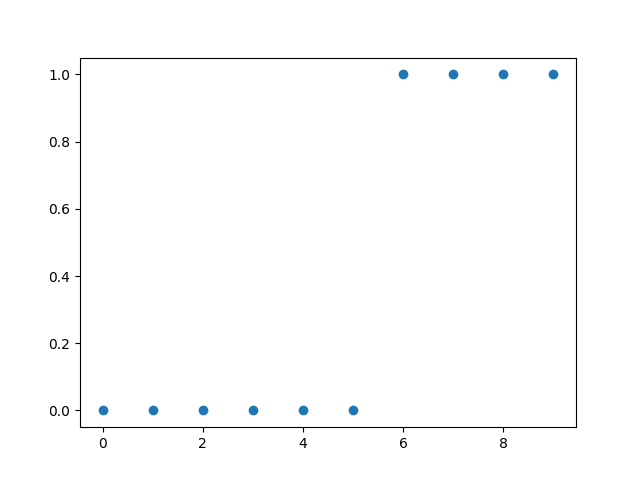
\includegraphics[scale=0.5]{figures/window-weights.png}
  \captionof{figure}{Window weights}
  \label{fig:window-weights}
\end{minipage}%
\begin{minipage}{.5\textwidth}
  \centering
      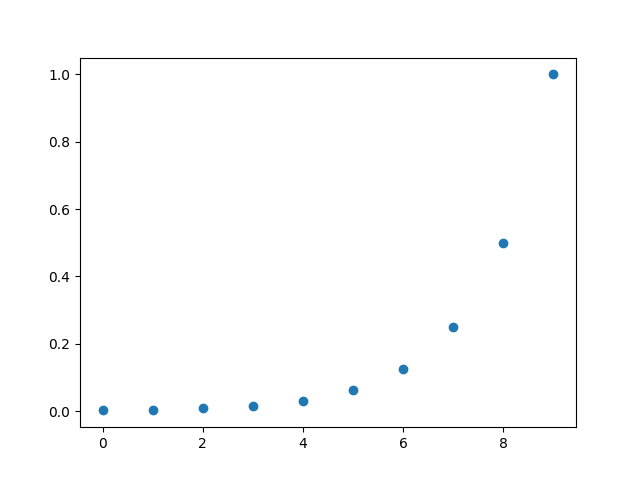
\includegraphics[scale=0.5]{figures/ema-weights.png}
  \captionof{figure}{EMA weights}
  \label{fig:ema-weights}
\end{minipage}
\end{figure}


EMAs are recursive: the EMA value at timestamp \textit{t} depends only on the EMA value at timestamp \textit{t-1}. This recursive property allows us to store only one EMA value and continuously update it for each new value val\textsubscript{t}, based on the following recursion formula:

\begin{definition}
EMA\textsubscript{t} = EMA\textsubscript{t-1} * $\lambda\delta\textsubscript{t}$ + val\textsubscript{t}
\label{def:ema}
\end{definition}

with $\lambda$ as a constant factor applied to the previous EMA value and $\delta\textsubscript{t}$ as the time passed between \textit{t} and \textit{t-1}. This $\lambda$ constant (0 < $\lambda \leq$ 1) is known as the smoothing coefficient. The smoothing or decay factor $\lambda$ is given by:
\begin{equation}
    \lambda = 2^{- \dfrac{1}{\tau}}
    \label{eq:ema-decay}
\end{equation}
where $\tau$ is the half-life of the EMA. The half-life $\tau$ controls how fast old events are forgotten as the smoothing factor depends on it. The half-life is the amount of time that it takes for an element to see its contribution or weight reduced to half. For instance, with $\tau = 1s$ we have $\lambda = 0.5$, which means for each 1s step we reduce the weights applied to each event by half. 

Note that it is also possible to express a tuple-based half-life, \textit{i.e.}, how many tuples or events must the EMA process before a certain element has its weight reduced by half. In this case, the definition does not take into account the time passed between events:
\begin{definition}
EMA\textsubscript{t} = EMA\textsubscript{t-1} * $\lambda$ + val\textsubscript{t}
\label{def:tuple-ema}
\end{definition}
For example, with a tuple-based half-life of $\tau = 1$ tuple, the smoothing factor is $\lambda = 0.5$, meaning for each new tuple all weights are reduced by half.

Definition \ref{def:ema} introduces the recurrence formula for time-based EMAs whereas Definition \ref{def:tuple-ema} works for tuple-based ones. In this Thesis we chose to work with tuple-based EMAs due to its simplicity but our approach can be adjusted to use time-based ones.